\chapter{AIXI}

\vspace{1em}
\hfill
\begin{minipage}[c]{0.55\textwidth}
\raggedleft
\small\itshape
Intelligence measures an agent's ability to achieve goals in a wide range of environments.\\[0.5em]
\upshape\footnotesize Shane Legg and Marcus Hutter, ``Universal Intelligence: A Definition of Machine Intelligence'' (2007)
\end{minipage}%
\hspace{0.5em}
\begin{minipage}[c]{0.12\textwidth}
% \includegraphics[width=\textwidth]{figures/ch08_aixi.png}
\end{minipage}
\vspace{1.5em}

\noindent Part I built one half of the picture. Part II built the other.

Part I was about prediction. Bayesian inference is the unique consistent calculus of belief. Solomonoff induction is what optimal prediction looks like once the prior problem is closed: weight every computable hypothesis by $2^{-|p|}$ where $p$ is the program producing it. The universal prior $M$ catches up to any computable distribution generating your data.

Part II was about decision. Expected utility maximization is the unique consistent calculus of choice. Reinforcement learning is what optimal decision looks like over time, with rewards and uncertainty. Function approximation lets the agent generalize from seen states to unseen ones; inductive biases are the engineering content of generalization.

Both halves are uncomputable in idealized form. Neither alone tells you what intelligence \emph{is}. This chapter combines them.

\section*{The setup}

Imagine an agent embedded in an unknown environment. The environment is some program $\mu$ that, given the agent's past actions, produces observations and rewards. The agent does not know which program $\mu$ is. It can only act, observe, and try to do well.

What should the agent believe about $\mu$? It should treat $\mu$ as a hypothesis to be inferred from data.

What is the right prior over $\mu$? Part I gave the answer: the universal prior. Weight every candidate environment-program by $2^{-K(\mu)}$, the cost of its shortest description.

What should the agent do? Part II gave the answer: pick the action that maximizes expected discounted reward, where the expectation is computed using the agent's current beliefs about $\mu$.

Combine these two answers and you get AIXI.

\section*{AIXI defined}

Let $h_t = a_1 o_1 r_1 \cdots a_t o_t r_t$ be the history of actions, observations, and rewards through step $t$. At step $t+1$, AIXI chooses the action

$$a_{t+1} = \arg\max_a \sum_{o, r} \sum_\nu 2^{-K(\nu)} \cdot \nu(o, r \mid h_t a) \cdot \big[r + \gamma \cdot V^*(h_t a o r)\big],$$

where $\nu$ ranges over all computable environments (more precisely, lower-semicomputable semimeasures), $\gamma$ is the discount factor, and $V^*$ is the best expected discounted return achievable from a given history. Each symbol is unpacked below; $V^*$ in particular is defined two paragraphs on, so read past it for now.

The two outer sums encode an expectation. The sum $\sum_{o, r}$ ranges over every possible next-step outcome: every (observation, reward) pair the environment could produce after the agent takes action $a$. The sum $\sum_\nu$ ranges over every candidate environment-program, weighted by its prior $2^{-K(\nu)}$. Together they marginalize jointly over what the true environment is and what its next response will be, producing the expected value of $r + \gamma V^*(h_t a o r)$ under AIXI's full posterior. The $\arg\max_a$ on the outside then picks the action whose expected value is largest.

The remaining symbols are string-valued and deserve a closer look. The notation $h_t a$ is the history-so-far with the candidate action appended: take everything that has happened through step $t$ and write $a$ on the right of it. The notation $h_t a o r$ extends the history one step further still, appending the resulting observation $o$ and reward $r$. The conditional $\nu(o, r \mid h_t a)$ then reads as follows: given the full history through step $t$ and given that the agent now takes action $a$, what probability does environment-program $\nu$ assign to the next observation being $o$ and the next reward being $r$? And $V^*(h_t a o r)$ is the optimal expected discounted return from the point at which the agent's history is exactly $h_t a o r$, after this hypothetical step has played out.

One design choice deserves naming. AIXI conditions on \emph{histories}, not on states. Chapter 6 worked with Markov decision processes, where the current state captured everything relevant about the past. AIXI does not assume a Markovian environment. The candidate environment-programs $\nu$ can have arbitrary internal structure and respond to any portion of the past, so the agent conditions on the full observable history. $V^*$ is recursive: unrolled, it considers every future trajectory each $\nu$ admits, with AIXI picking the best action at each future step.\footnote{The equation is therefore self-referential. $V^*$ is the value of acting optimally from a history, and acting optimally means applying this very action-selection rule at every subsequent step, so $V^*$ appears, implicitly, on both sides. It is a fixed point: the value function consistent with choosing the best action everywhere downstream. This is the Bellman optimality equation of Chapter 6, lifted from a single known environment to AIXI's posterior mixture over all computable environments.}

This may seem to backtrack from Chapter 7, which insisted that real systems need state representations: features, neural-network embeddings, learned compressions of the past. AIXI throws all of that away and conditions on the raw history.

It does so on purpose. The representation work has not disappeared; it has moved into the prior. Each candidate environment-program $\nu$ is, in effect, its own way of organizing the past: $\nu$'s internal state-tracking is its representation of the history. Different $\nu$'s use different representations. The universal prior $2^{-K(\nu)}$ weights them all, with simpler representations getting more weight.

So AIXI does not lack representations. It runs all of them in parallel, weighted by simplicity, and lets the data sort out which one is correct. A practical agent commits to a finite, manageable set of representations. It might use one architecture, or a small ensemble, or a mixture of experts that routes different inputs to different sub-networks, or a multi-head attention module that effectively learns several representations within a single architecture; in every case the set is finite and chosen at design time. That is the architecture choice from Chapter 7. AIXI does not commit to any such set. It weights every computable representation. Refusing to commit is what makes it universal. It is also what makes it uncomputable. On the inductive-bias trade-off curve of Chapter 7, AIXI sits all the way at the universal end. Every practical agent sits to the left, having committed to a finite set of biases in exchange for being something that can actually run.

The equation is dense. Figure~\ref{fig:aixi-loop} unpacks the pieces and shows the loop they describe.

\begin{figure}[h]
\centering
\begin{tikzpicture}[
  scale=1.0,
  every node/.style={align=center, font=\small},
  >=Stealth
]
  \node[draw, thick, fill=blue!20, rectangle, rounded corners, minimum width=3.5cm, minimum height=2.5cm, text width=3.2cm] (agent) at (0, 0) {\textbf{AIXI}\\[0.3em]\scriptsize belief over environment-programs $\nu$, weighted by $2^{-K(\nu)}$};

  \node[draw, thick, fill=gray!15, rectangle, rounded corners, minimum width=3.5cm, minimum height=2.5cm, text width=3.2cm] (env) at (8, 0) {\textbf{Environment}\\[0.3em]\scriptsize true program $\mu$\\(unknown to AIXI)};

  \draw[->, thick, blue] ([yshift=0.6cm]agent.east) -- ([yshift=0.6cm]env.west);
  \node[font=\scriptsize, blue!50!black, anchor=south, align=center] at (4, 0.7) {action $a$ that maximizes\\expected discounted reward\\under the universal prior};

  \draw[->, thick, red] ([yshift=-0.6cm]env.west) -- node[below, font=\scriptsize, red!50!black, midway] {observation $o$, reward $r$} ([yshift=-0.6cm]agent.east);

  \node[font=\scriptsize, anchor=south, gray] at (4, 1.8) {after each step, AIXI updates its weighted belief over $\nu$};
\end{tikzpicture}
\caption{The AIXI loop. AIXI maintains a posterior over environment-programs $\nu$, weighted by their universal prior $2^{-K(\nu)}$ and conditioned on the history so far. At each step, it picks the action whose expected discounted return is highest under this posterior, marginalizing over which $\nu$ is the true environment. The action is taken; the environment responds with observation and reward; AIXI updates its posterior; the loop continues.}
\label{fig:aixi-loop}
\end{figure}

In plain language: AIXI considers every computable theory of what the environment might be. It weights each theory by how short it is to describe. It computes, for each candidate action, the expected reward (discounted, summed over time) the action would produce, taking the expectation over its weighted theories of the environment. It picks the action whose expected reward is highest.

Three pieces, each from elsewhere in the book:

\begin{itemize}
\item The \textbf{prior} $2^{-K(\nu)}$ over environments comes from Solomonoff (Part I, Ch 4).
\item The \textbf{posterior} is Bayesian updating on the observed history (Part I, Ch 1).
\item The \textbf{decision rule} is expected utility maximization over discounted future reward (Part II, Chs 5-6).
\end{itemize}

AIXI is the synthesis. Nothing in the equation is new; the move is putting it all in one place.

\section*{What AIXI achieves}

Hutter (2000, 2005) proved several optimality properties.

\textbf{Self-optimizing in the limit.} For any computable environment $\mu$, AIXI's expected return converges to the expected return of an agent that knows $\mu$ and acts optimally in it. In the long run, AIXI does as well as it could have done with full knowledge.

\textbf{Pareto-optimal.} No other agent dominates AIXI across all computable environments. Any other agent that does better than AIXI in some environment necessarily does worse in another.

\textbf{Universal.} AIXI's optimality holds for every computable environment, not just a particular one. The convergence is at the rate determined by $K(\mu)$: the simpler the true environment, the faster AIXI catches up.

The strength of these properties is hard to overstate. AIXI is provably the best one can do, in a precise sense, across the entire class of computable environments. It does not require knowing what kind of environment one is in. It does not require a hand-designed inductive bias. It just runs Bayesian inference with the universal prior and picks the action that maximizes expected discounted reward.

If you could build AIXI, it would be the agent.

\section*{The catch}

You cannot build AIXI.

AIXI inherits all of Solomonoff's uncomputability and adds more. To compute the action at each step:

\begin{itemize}
\item You have to enumerate every computable environment-program. Infinitely many.
\item You have to determine which ones halt and produce coherent outputs. Halting problem.
\item You have to compute, for each, the expected discounted reward conditional on each candidate action. Each conditional expectation involves looking arbitrarily far into the future under that environment.
\item You have to integrate over all of this. Infinite sums, infinite expectations, no closed form.
\end{itemize}

The equation is a definition, not a computation. AIXI is, in the formal sense, a lower-semicomputable function. You can approximate it from below, given infinite time. You cannot compute it exactly in finite time.

This is not a flaw to be engineered around. It is what makes AIXI universal. Any computable approximation is necessarily restricted in some way, and is therefore not optimal across all computable environments. Optimality across all of them \emph{requires} a definition that exceeds what any finite computation can deliver.

\section*{Bounded approximations}

Real AI systems are bounded approximations of AIXI, in roughly the sense that real physical machines are bounded approximations of Turing machines. They share the conceptual structure but trade universality for tractability.

A few explicit attempts at AIXI approximation:

\textbf{AIXItl.} Hutter's own time- and length-bounded approximation. Restrict to programs of length at most $\ell$ and run them for at most $t$ steps. The result is computable but exponentially slow in $\ell$ and $t$. For toy problems it works; for anything realistic it does not.

\textbf{MC-AIXI-CTW.} Veness, Ng, Hutter, Uther, and Silver (2011) replaced the environment-program enumeration with Context Tree Weighting (CTW), a mixture model over Markov chains of bounded depth. They used Monte Carlo Tree Search for the action selection. The result is computable in practice and plays simple games (Pac-Man, partial-observable Tic-Tac-Toe) at a competent level.

\textbf{Modern deep reinforcement learning.} DQN, AlphaZero, MuZero, and their successors are also bounded approximations of AIXI in this loose sense. They use neural networks to approximate value functions and policies; they use experience replay or self-play to approximate Bayesian updating; they use restricted prior families (the inductive biases of Chapter 7) rather than the universal prior.

None of these approximations is AIXI. They share its structural commitments (predict, weight by some prior, pick the highest-EU action) but use specific parametric machinery in place of the universal apparatus.

Figure~\ref{fig:aixi-ladder} shows the relationship.

\begin{figure}[h]
\centering
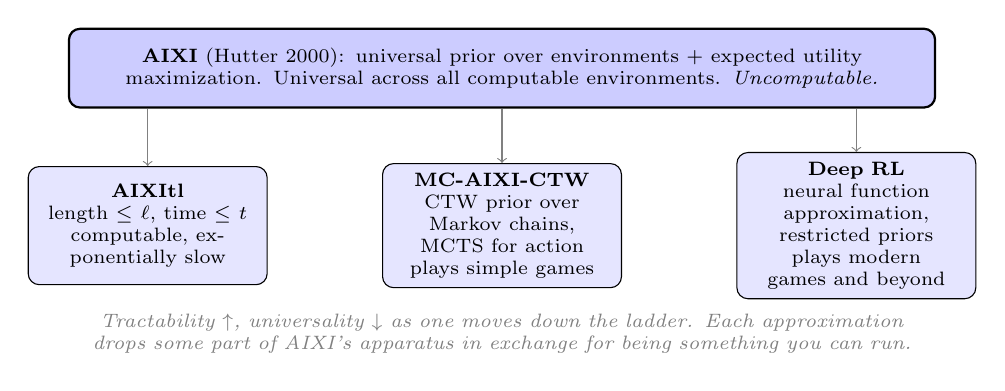
\begin{tikzpicture}[scale=1.0, every node/.style={align=center, font=\scriptsize}]
  % Top: AIXI
  \node[draw, thick, fill=blue!20, rounded corners, minimum width=11cm, minimum height=1cm, text width=10.5cm] (aixi) at (5.5, 5.5) {\textbf{AIXI} (Hutter 2000): universal prior over environments + expected utility maximization. Universal across all computable environments. \emph{Uncomputable.}};

  % Below AIXI: bounded approximations
  \node[draw, fill=blue!10, rounded corners, minimum width=3cm, minimum height=1.5cm, text width=2.8cm] (aixitl) at (1, 3.5) {\textbf{AIXItl}\\\scriptsize length $\leq \ell$, time $\leq t$\\\scriptsize computable, exponentially slow};

  \node[draw, fill=blue!10, rounded corners, minimum width=3cm, minimum height=1.5cm, text width=2.8cm] (mcaixi) at (5.5, 3.5) {\textbf{MC-AIXI-CTW}\\\scriptsize CTW prior over Markov chains, MCTS for action\\\scriptsize plays simple games};

  \node[draw, fill=blue!10, rounded corners, minimum width=3cm, minimum height=1.5cm, text width=2.8cm] (deepRL) at (10, 3.5) {\textbf{Deep RL}\\\scriptsize neural function approximation, restricted priors\\\scriptsize plays modern games and beyond};

  % Arrows
  \draw[->, gray] (aixi.south -| aixitl.north) -- (aixitl.north);
  \draw[->, gray] (aixi.south -| mcaixi.north) -- (mcaixi.north);
  \draw[->, gray] (aixi.south -| deepRL.north) -- (deepRL.north);

  % Bottom label
  \node[font=\scriptsize, anchor=north, text width=11cm, align=center, gray] at (5.5, 2.5) {\emph{Tractability $\uparrow$, universality $\downarrow$ as one moves down the ladder. Each approximation drops some part of AIXI's apparatus in exchange for being something you can run.}};
\end{tikzpicture}
\caption{AIXI and its bounded approximations. AIXI sits at the top: universal across all computable environments, but uncomputable. Below it are progressively more tractable approximations, each restricting the prior, the planning horizon, the function class, or all three. Deep RL systems are the dominant approximations in 2026; they trade nearly all of AIXI's coverage for the ability to run on real problems with real data.}
\label{fig:aixi-ladder}
\end{figure}

\section*{The reference point}

If AIXI cannot be built, why does it matter?

It matters because it is the reference point. Optimal intelligence under the Church-Turing thesis is, mathematically, AIXI. We have a definition. We have a target. We have a way of comparing any candidate agent to the ideal: how close is it, and along what dimensions does it fall short?

Compare the situation in physics. Ideal gases do not exist; no real gas perfectly obeys the ideal gas law. But the ideal gas law is the reference point. Real gases are described as departures from it: van der Waals corrections, non-ideal behavior at high pressures, real-gas equations of state. The ideal gives the language for talking about the real.

AIXI plays the same role for intelligence. We do not build AIXI; we build agents that depart from AIXI in specific ways, and the gap between them and AIXI is the gap we have to understand.

The remaining chapters are about that gap. Three things make the gap real and consequential:

\begin{itemize}
\item The agent's prior is not the universal prior. It is a bounded inductive bias chosen for tractability (the architecture choice from Chapter 7). What the agent learns depends on what its bias lets it learn.
\item The agent's planning horizon is finite. It cannot compute expected returns arbitrarily far into the future. It uses approximations, heuristics, learned value functions.
\item The agent's reward function is not the true objective. It is a proxy that the designer has written down, hoping the proxy captures what they actually want. This is the specification problem, and it is the subject of Part III.
\end{itemize}

\section*{Where this leaves you}

Part II closes here.

You now have a complete theory of optimal agency. Bayesian inference is the unique consistent calculus of belief (Chapter 1). The universal prior is the unique optimal starting point for that inference (Chapter 4). Expected utility maximization is the unique consistent calculus of decision (Chapter 5). The state-action-reward loop is the temporal generalization (Chapter 6). Function approximation and inductive biases are how bounded systems generalize (Chapter 7). And AIXI is the synthesis (this chapter).

The mathematics is complete. It is also uncomputable, parameter-free except for the reward function, and silent on the question of which reward function is the right one.

The next chapter takes up that question. Part III is the specification problem: where utility functions come from, why specifying them is harder than it looks, and what the consequences are when the specification fails. Reward modeling is where the alignment problem lives, and the alignment problem is where the consequences of the gap between AIXI and any buildable system become real.

Part III opens with reward modeling, in idealized settings, before Part IV moves to the empirical reality of actual systems.

The book has built half of its argument. The other half follows.
